% Template authors: Mateusz Grochowski, Bartosz Bizoń
% Github repository: https://github.com/Gromate/latex-template-pk

% Set document class
\documentclass[11pt,a4paper]{article}

%% Import packages

% Provides support for multilingual documents, specifically Polish in this case.
\usepackage[polish]{babel}

% Enables Polish-specific typographic rules and hyphenation.
\usepackage{polski}

% Ensures proper encoding of fonts, especially for Polish characters.
\usepackage[T1]{fontenc}

% Essential for advanced mathematical typesetting.
\usepackage{amsmath}

% Allows the inclusion of graphics (e.g., images) in the document.
\usepackage{graphicx}

% Enhances table formatting with additional column types and alignment options.
\usepackage{array}

% Adds hyperlinks to the document, with all links colored black.
\usepackage[colorlinks=true, allcolors=black]{hyperref}

% Improves the quality of tables with professional-looking horizontal rules.
\usepackage{booktabs}

% Provides additional text symbols and degree symbols.
\usepackage{textcomp, gensymb}

% Provides better control over the placement of floating objects like figures and tables.
\usepackage{float}

% Enables subfigures with individual captions within a single figure environment.
\usepackage{subcaption}

% Ensures proper handling of quotations, especially in multilingual documents.
\usepackage{csquotes}

% Allows URLs to break across lines, improving readability in references.
\usepackage{xurl}

% Customizes the formatting of the table of contents, list of figures, and list of tables.
\usepackage{tocloft}

% Enhances captions for figures, tables, and other floating environments.
\usepackage{caption}

% Provides bold math symbols for use in mathematical expressions.
\usepackage{bm}

% Improves text alignment options, including ragged-right and ragged-left.
\usepackage{ragged2e}

% Creates tables with adjustable column widths, useful for complex layouts.
\usepackage{tabularx}

% Allows the inclusion of external PDF pages in the document.
\usepackage{pdfpages}

% Provides a way to include formatted source code listings in the document.
\usepackage{listings}

% Enables the use of colors in the document, useful for highlighting text or code.
\usepackage{xcolor}

% Offers syntax highlighting for source code, often used with the `minted` environment.
% To use it on windows you need to install Python and libraries:
% - Pygments
% - latexminted
\usepackage{minted}

% Ensures the first paragraph after a section title is indented, following Polish typographic conventions.
\usepackage{indentfirst}

% Set document style
\renewcommand{\arraystretch}{1.2} % opcjonalnie zwiększa odstęp pionowy między wierszami
\usepackage[a4paper,top=2.5cm,bottom=2.5cm,left=2.5cm,right=2.5cm,marginparwidth=1.75cm]{geometry}
\renewcommand{\baselinestretch}{1.25} 

% Configure section styles
\renewcommand\thesection{\arabic{section}.}
\renewcommand\thesubsection{\thesection\arabic{subsection}.}
\renewcommand\thesubsubsection{\thesection\arabic{subsection}.\arabic{subsubsection}.}

% Configure tables, figures
\renewcommand{\thetable}{\thesection\arabic{table}}
\renewcommand{\thefigure}{\thesection\arabic{figure}}

% Configure listings
\renewcommand{\thelisting}{\thesection\arabic{listing}}
\lstset{
  basicstyle=\ttfamily, % Use a~ typewriter font
  columns=fullflexible, % Allow line breaking
  breaklines=true,       % Enable line breaking
  backgroundcolor=\color{white}, % Background color
}

% Configure caption styles
\captionsetup[figure]{name=Rys, labelsep=period, font=it}
\captionsetup[listing]{font=it}
\captionsetup[table]{font=it}

% Use TimesNewRoman font
\usepackage{times}

% Customize the Table of Contents
\renewcommand{\cftsecfont}{\bfseries}  % Section titles in bold
\renewcommand{\cftsecpagefont}{\bfseries} % Section page numbers in bold
\setlength{\cftbeforesecskip}{0pt} % Space between sections in the ToC
\setlength{\cftsecindent}{0pt} % No indentation for sections
\setlength{\cftsubsecindent}{16pt} % Indent subsections by 20pt
\setlength{\cftbeforesubsecskip}{0pt}

% Add dots to Table of Contents
\renewcommand{\cftsecleader}{\textbf{\cftdotfill{\cftdotsep}}} % Dots for sections
\renewcommand{\cftsubsecleader}{\cftdotfill{\cftdotsep}} % Dots for subsections
\renewcommand{\cftdotsep}{0.5}

% Add command for inline code \inlinecode
\newcommand{\inlinecode}[1]{%
  \texttt{%
    % set flexible interword space
    \setlength{\spaceskip}{0.5em plus 1em minus 0.1em}%
    % add some space with not as much flexibility, but only
    % if some space precedes
    \ifdim\lastskip>0pt \unskip\hspace{0.5em plus 0.5em minus 0.1em}\fi
    #1
  }
}

\begin{document}

\begin{titlepage}
   \begin{center}
       \begin{table}
        \centering
        \begin{tabular}{ccc}
        \begin{minipage}{.1\textwidth}
            \raggedleft
            
\includegraphics[width=1\linewidth]{media/logo-pk.png}
        \end{minipage}
         &  
        \begin{minipage}{.7\textwidth}
        \centering
            \large \textbf{POLITECHNIKA KRAKOWSKA im. T. Kościuszki}\break
            Wydział Mechaniczny \break
            \large \textbf{Katedra Informatyki Stosowanej}
        \end{minipage}
        & 
        \begin{minipage}{.1\textwidth}
            \raggedright
            
\includegraphics[width=1\linewidth]{media/logo-mech.png}
        \end{minipage}
        \\
        \end{tabular}
        \end{table}

    \begin{minipage}{12cm}
    \vspace*{1cm}
    \raggedright
        \large Kierunek studiów: \break
        \large Specjalność: \break
    \end{minipage}
    \vspace*{1cm}

    \large STUDIA STACJONARNE
    \vspace*{1cm}
    
    \textbf{\Huge PRACA DYPLOMOWA} \break
    \LARGE INŻYNIERSKA
            
    \vspace{1.5cm}

    \textbf{\Large Autor}

    \vspace{1.5cm}

    \large Temat pracy dyplomowej w języku polskim \break 

    Temat pracy dyplomowej w języku angielskim

    \vspace*{1.5cm}

    Promotor: \break
    Tytuł/stopień naukowy \textbf{Imię i nazwisko}
    \vfill

    Kraków, rok akad. 2024/2025

    \vspace{1cm}
    
            
   \end{center}
\end{titlepage}

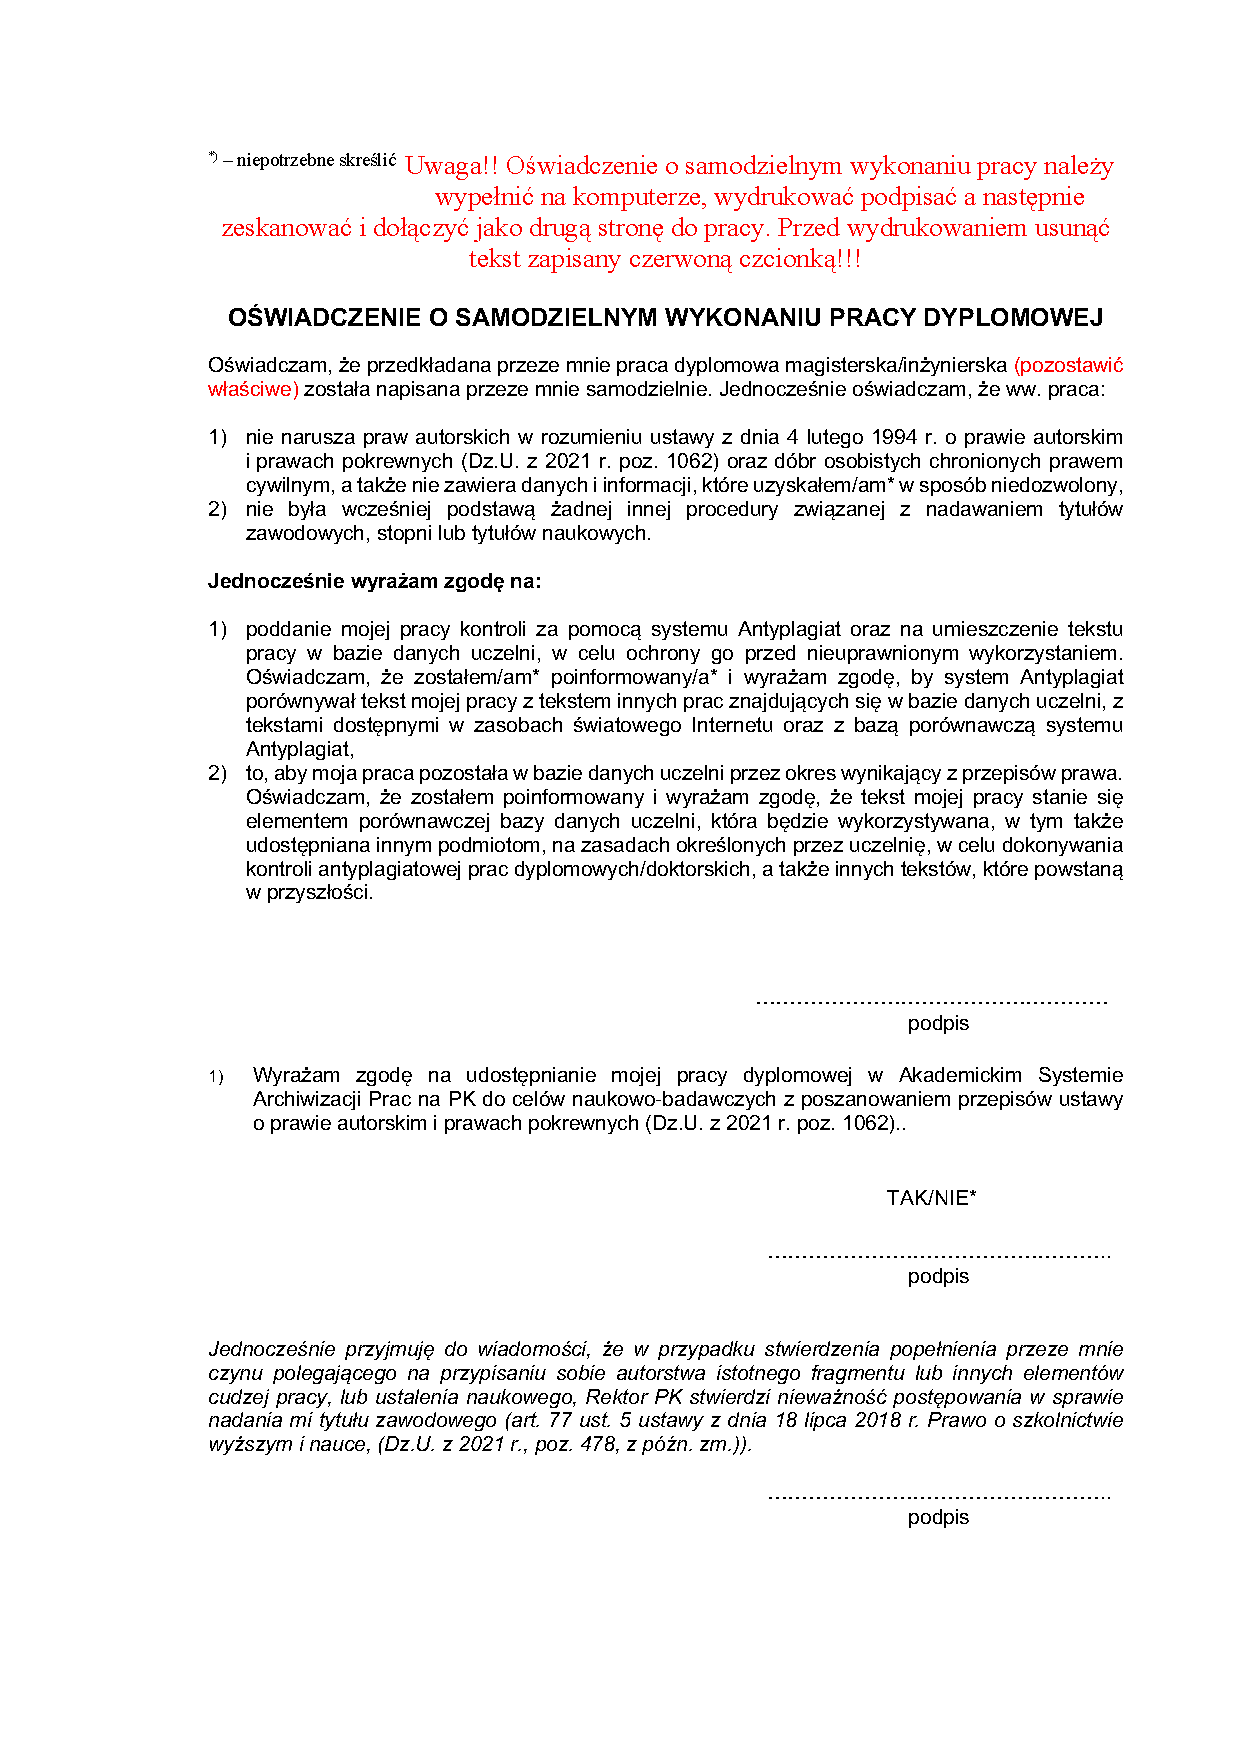
\includepdf[pages=-]{media/zaswiadczenie-sample.pdf}

\renewcommand{\contentsname}{\LARGE \normalfont \MakeUppercase{Spis treści} (Times New Roman 16)}

{\fontsize{12}{16}\selectfont
\tableofcontents
}

\newpage

% You can start writing document here
% Example sections are presented below
% Zacznij pisać tutaj
% Przykładowe rozdziały zostały przedstawione poniżej

\section{Cel i zakres pracy (Styl Nagłówek 1, Times New Roman 14)}
\paragraph{}
(Styl Standardowy, Times New Roman 11 lub Arial 11, odstęp między liniami tekstu 1.25 wiersza, wcięcie pierwszego wiersza: 0,6). W rozdziale „Cel i zakres pracy” należy przedstawić jasno, co jest przedmiotem pracy. Wyjaśnić cel oraz podać czynności, które zostały wykonane, aby ten cel został osiągnięty. W rozdziale tym można opisać z czego praca będzie się składać, np.: 
Niniejsza praca dyplomowa składać się będzie z dwóch głównych części. Pierwsza z nich poświęcona zostanie omówieniu zagadnień teoretycznych, związanych z wykorzystaniem energii słonecznej, a w szczególności … Druga część tej pracy związana będzie bezpośrednio z wykonywanym projektem.
Jeżeli zostało użyte oprogramowanie przy realizacji pracy należy to oprogramowanie wymienić. Rozdział „Cel i zakres pracy” powinien zając maksymalnie jedną stronę. 

\newpage

\section{Wstęp}
\paragraph{}
Tekst pracy należy napisać czcionką Time New Roman 11 lub Arial 11, odstęp 1.25 wiersza, wcięcie pierwszego wiersza: 0,63 (Styl Standardowy). Do całości pracy zastosować wyjustowanie akapitów, lewy margines ma wynosić 3.5 cm natomiast pozostałe marginesy 2.5 cm. Przy drukowaniu pracy należy uwzględni fakt, że jeden z egzemplarzy ma zostać wydrukowany dwustronnie i oprawiony w miękkie oprawki (marginesy lustrzane). Rozdziały główne pracy powinny być umieszczone na następnej (nowej) stronie.

\newpage

\section{Układ graficzny pracy}

\indent Przy pisaniu pracy obowiązuje styl bezosobowy tak jak pokazują to poniższe przykłady:  

\noindent Wpływ zachmurzenia na gęstość strumienia promieniowania słonecznego \underline{przedstawiono} na rysunku \ref{fig:azymut-slonca} – \textbf{poprawnie}

\noindent Wpływ zachmurzenia na gęstość strumienia promieniowania słonecznego \underline{przedstawia} rysunek \ref{fig:azymut-slonca} – \textbf{poprawnie}

\noindent Wpływ zachmurzenia na gęstość strumienia promieniowania słonecznego \underline{przedstawiłem} na rysunku \ref{fig:azymut-slonca} – \textbf{niepoprawnie}

\begin{figure}[H]
    \centering
    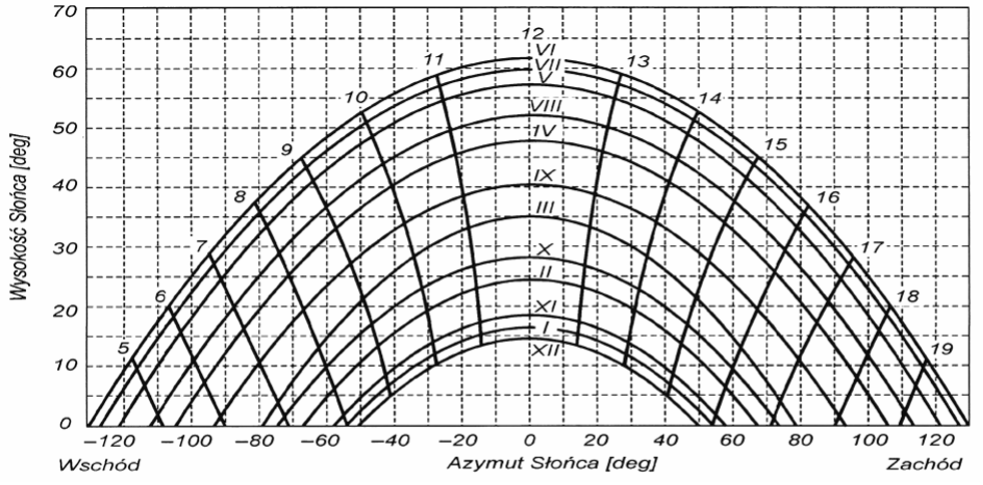
\includegraphics[width=0.75\linewidth]{media/azymut_slonca.png}
    \caption{Wysokość i azymut Słońca dla 52°N}
    \label{fig:azymut-slonca}
\end{figure}

Styl RYS, Times New Roman 11, kursywa, odstęp pomiędzy wierszami pojedynczy. W podpisach rysunków nie dajemy kropki na końcu

\subsection{Wzory}

Jeżeli występują w tekście \cite{ksiazka} wzory należy je numerować oraz podać opis wielkości w nich występujących. Wzory należy wyśrodkowywać a numerowanie worów wyrównywać do prawej krawędzi tak jak przedstawia to poniższy przykład. Zmienne we wzorach powinny być napisane kursywą. Wzór jest częścią zadania, obowiązują w związku z tym zasady interpunkcji.   
Przykład:
Chwilowa wartość natężenia promieniowania jest parametrem, który wylicza się z zależności:
	  (Styl Wzór),	(3.1)
gdzie:
opt - sprawność optyczna kolektora,
UL- współczynnik całkowitych strat kolektora, [W/m2K],
T- różnica temperatur pomiędzy czynnikiem solarnym a otoczeniem, [K].

\subsection{Rysunki tabele i listingi}

\paragraph{}
Rysunki oraz tabele (tylko dobrej jakości, min. 300dpi) występujące w tekście należy wyśrodkowywać. Każdy rysunek oraz tabela musi zawierać numer oraz podpis. Podpis umieszcza się pod rysunkiem oraz nad tabelą, tak jak to przedstawiają poniższe przykłady. Odstęp pomiędzy tekstem a rysunkiem wynosi jedną linię. Uwaga! Nie można wstawiać do pracy rysunków oraz tabel bez ich opisu/komentarza w tekście. Rysunek lub tabela pozbawione komentarzy w tekście są bezwartościowe i obniżają jakość pracy. 
Przykład: Wysokość i azymut Słońca we wszystkich porach roku przedstawia rysunek 2.1. Gęstość strumienia promieniowania zależy od zachmurzenia co ilustruje rys.2.2.

\subsubsection{Rysunek}
\begin{figure}[H]
    \centering
    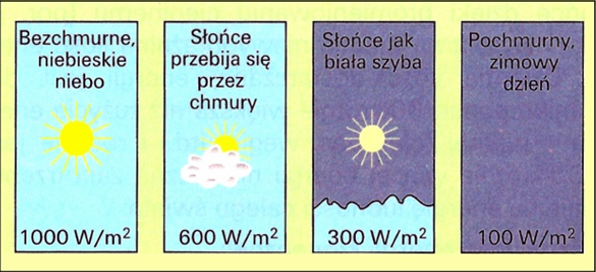
\includegraphics[width=0.75\linewidth]{media/zachmurzenie.png}
    \caption{Wpływ zachmurzenia na gęstość strumienia promieniowania słonecznego}
    \label{fig:zachmurzenie}
\end{figure}

Wstawiane do pracy rysunki, schematy, wykresy, zdjęcia są traktowane jak rysunki i nie rozróżnia się ich w podpisach. Pomimo tego, że wstawiany jest wykres podpisywany jest on jako kolejny rysunek. Rysunki umieszcza się w pracy przez wstawienie z pliku *.jpg.
Numeracje rysunków, tabel oraz wzorów przeprowadza się w obrębie głównych rozdziałów. Wyniki obliczeń dla poszczególnych miesięcy przedstawia tabela 2.1.

\subsubsection{Tabela}
\begin{table}[H]
\centering
\begin{tabularx}{\textwidth}{|c|X|X|X|X|X|}
\hline
Miesiąc & Temperatura zimnej wody w punkcie czerpalnym \(\boldsymbol{t_w}\left[ \boldsymbol{^\circ C} \right]\) 
& Entalpia wody zimnej \(\boldsymbol{i_w}\left[kJ/kg\right]\) 
& Dzienny rozbiór \(\boldsymbol{O^{d}_{c.w.u.}} \left[dm^3\right]\) 
& Udział c.w.u. w wodzie zmieszanej \(\dfrac{\boldsymbol{O^{d}_{c.w.u.}}}{\boldsymbol{O^{d}_{zm}}}\) 
& Średnia ilość energii do przygotowania c.w.u. w ciągu doby \(\boldsymbol{Q^{d}_{c.w.u.}} \left[kWh\right]\) \\

\hline
Styczeń     &  &  &  &  &  \\
\hline
Luty        &  &  &  &  &  \\
\hline
Marzec      &  &  &  &  &  \\
\hline
Kwiecień    &  &  &  &  &  \\
\hline
Maj         &  &  &  &  &  \\
\hline
Czerwiec    &  &  &  &  &  \\
\hline
Lipiec      &  &  &  &  &  \\
\hline
Sierpień    &  &  &  &  &  \\
\hline
Wrzesień    &  &  &  &  &  \\
\hline
Październik &  &  &  &  &  \\
\hline
Listopad    &  &  &  &  &  \\
\hline
Grudzień    &  &  &  &  &  \\
\hline
\end{tabularx}
\end{table}

\subsubsection{Listing}
\begin{listing}[H]
\begin{minted}[breaklines]{bash}
curl -X 'GET' \
  'http://{address}/api/Info/GetAllAsync' \
  -H 'accept: */*'
\end{minted}
\caption{Przykładowe zapytanie API w celu uzyskania informacji.}
\label{listing:get-all-req}
\end{listing}

\subsection{Cytowania}

W przypadku cytowania \cite{greenwade93} fragmentów tekstów, tabel, rysunków lub wzorów z literatury należy zaznaczyć autora tego cytowania w tekście pracy.
Sposób pierwszy: Cytowanie poprzez umieszczenie odpowiedniego numeru w nawiasie kwadratowym. Powołanie na literaturę umieszcza się po cytowanym fragmencie teksu przed kropką np.: Na skutek procesów zachodzących w atmosferze, do powierzchni Ziemi dociera jedynie 39-45\% promieniowania pozaatmosferycznego w skali roku [10].  - poprawnie    
Na skutek procesów zachodzących w atmosferze, do powierzchni Ziemi dociera jedynie 39-45\% promieniowania pozaatmosferycznego w skali roku. [10]  - niepoprawnie    
Sposób drugi: Cytowanie poprzez powołanie się na autorów cytowanej pracy oraz roku publikacji pracy np.: Nowak i Kowalski (2009) w swojej pracy prezentują … 
Jeżeli autorami pracy są więcej niż dwie osoby należy użyć w cytowaniu tylko nazwiska pierwszego autora np.: Nowak i inni (2010) w swojej pracy prezentują …
Jeżeli ci sami autorzy (lub autor) w jednym roku wydali kilka publikacji, które są w pracy cytowane należy po roku cytowanej publikacji dodać jeszcze literę zgodnie z kolejnością umieszczenia publikacji w wykazie literatury np.: Nowak (2011a) oraz Nowak (2011c) w swoich pracach przedstawia …

\newpage

\section{Wnioski}

We wnioskach należy w przejrzysty sposób podsumować pracę, napisać czy założony cel pracy został osiągnięty i w jakim stopniu. Jeżeli praca ma charakter projektu, autor powinien podać zalecenia projektowe wynikające z przeprowadzonych obliczeń/analiz. Jeżeli z pracy wynikają wnioski przyszłościowe należy je wymienić. Należy użyć stylu, rozmiaru czcionki i odstępu takich jak w całej pracy.

\newpage

\bibliographystyle{unsrt}
\bibliography{sample}
\addcontentsline{toc}{section}{Literatura}

\newpage

\newcommand{\summaryName}{Summary}

\begin{center}
\section*{\Large\textbf{\summaryName}}
\end{center}
\addcontentsline{toc}{section}{\summaryName}

W tym miejscu należy zamieścić streszczenie pracy w języku angielskim o objętości min. 2500 znaków ze spacjami.

\end{document}
